\chapter{System Design}

The complete work presented here can be divided into several parts right from
taking in a topic as input, finding out relevant documents, tagging words as
probable answer words, and eventually generating questions from it.

\begin{figure}
	\caption{Architecture of Model}
	\centering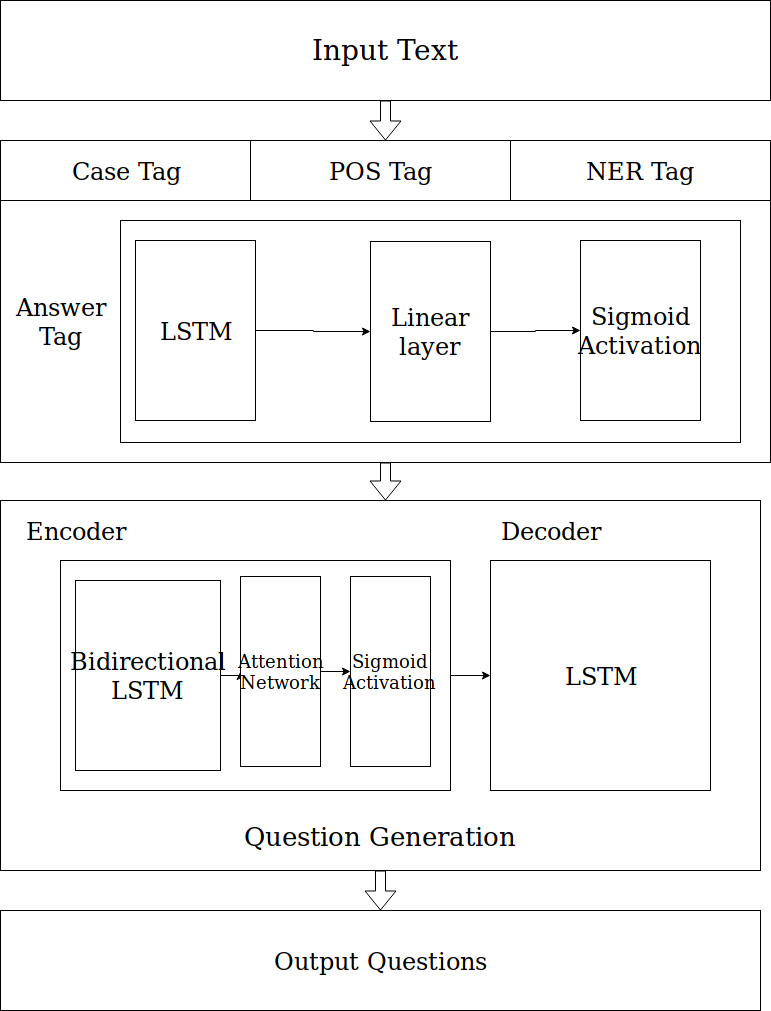
\includegraphics[width=10cm]{5.png}
\end{figure}

\section{Topic Input \& Data gathering}

Initially, the user shall enter his/her topic of interest into the software. The
software shall then crawl the web and gather links to various web pages relevant
to the topic given by the user. On getting the links, further the software shall
scrape those links and parse the HTML pages to get the information content in
those web pages. 
However, all the content received can be classified into three parts. The first
part consists of markup language tasks and syntax, the second part shall contain
data unrelated to the topic of interest, and the third shall be the data which
is useful and relevant both to the topic of interest. The data classified into
the first part, is removed by searching for markup language tasks in the
obtained data. On finding such tags, the lines containing such tags shall be
eliminated from the useful data text. For identifying data in the second part,
the semantic meaning of the words and the web page from where the data has been
input is taken into consideration. Thus eventually the system has data which can
be used for generating questions on the users topic of interest. 

\section{Pre processing block}

The processing block consists of four independent tasks.
The output of each of these four tasks works as features for the question
generation algorithm. The four tasks and their work can be summarized as follows -

\begin{enumerate}

\item Case Tagging - This feature determines whether the first
letter of the word is in lower or upper case. The output of this case thus
determines whether the word is the starting word of the context. In quite a few
cases, the starting word of the context dominates in meaning, and hence has been
considered as a feature in the problem.

\item NER Tagging - The 7 set Stanford NER Tagging is used in the system. The
NER Tagging helps in finding out the type of a noun to which the word belongs, i.e if it is a place, a
date or a person. Depending on the tag different kinds of 'Wh' questions are created and hence
the feature is of great significance in the problem.

\item POS Tagging - POS tags are important in generating patterns based on their
frequency in the contexts. Frequently occuring series of consecutive POS tags
that form answer words in the training sentences are most probable to be the
best sources for generating questions in test contexts as well.

\item Answer Words -
	This feature is the most important of all the four features. This
	feature talks of whether the word in consideration is an answer
	word or not, in the question to be formed. Only those words that
	are answer words are given paramount importance in the question
	generating process. 
	So to achieve this goal, different rule based algorithms are
	used depending on the type of questions to be formed

	\begin{enumerate}

	\item Fill in the blanks \& One Word Answers: In this question type, a
	factual important sentence is chosen from the input text. NER
	Tags of the words in this sentence are found out. Through our
	experimentation it was found out that consecutive words with
	same NER tags are a good fit as probable answer words. It is
	also ensured that the tags of such probable answer words do not
	belong to the ‘OTHER’ category.

	\item Subjective Questions: To generate ‘Subjective Questions’,
	possible patterns which lead to subjective questions were
	researched in the dataset. On research, words like ‘because’,
	‘means’, ‘states that’, ‘defines’, etc were identified as words
	whose sentences had content for generating subjective questions.
	The words in a sentence following these special words were
	tagged as possible answer words.

	\item Questions based on English Language: The software offers a
	special feature for improving students language skills. Once the
	content collection phase is completed, the system identifies
	difficult and rarely used words in the passage. On
	identification of such words, a user is presented with the
	meanings of such words and asked to identify the special word in
	the passage. Conversely, a user may also be provided with a word
	opposite in meaning to the special word, and would then be asked
	to identify the special word selected by the system. The tasks
	of identifying special words, the word meanings and words
	opposite in meaning to the given word are achieved using the
	word net library.

	\end{enumerate}

	Some machine learning models using RNNs have been explored for
	tagging purpose the answer words. These approaches are aimed at
	tagging answer words for forming all types of question mentioned
	above. They are discussed in Section : Machine Learning
	Approach.

\end{enumerate}

In order to achieve this goal, a model containing a LSTM and dense layers is
developed. The output of the model is binary string which is 1 for the Answer Tag
and 0 for non answer words. The output of this preprocessing subsystem is fed to the Question Generation Algorithm subsystem as input. 

\section{Question Generation - Algorithm}

The Question Generation Algorithm performs three major tasks - 

\begin{enumerate}

\item Fill in the Blanks: To create Fill In The Blanks questions, all the words that
are marked as Answer tag are made blank.

\item Synonym and Antonym words are asked directly.
\item Basic tense filling grammer is generated by entering blank in the verb part of
the sentence and the base word is provided in brackets.

\item Subjective and One word WH Questions is generated by passing the preprocessed
sentence to QG-Net model. The QG-Net model contains the following parts and each
is explained below:

\begin{itemize}

	\item \textbf{Context Reader and Encoder}

Context reader is a bi-directional long short-term memory (bi-LSTM) network with
		600 hidden layers. Bi-LSTM processes the input words in both the
		forward and backward direction. Encoder creates context word
		vectors from the preprocessed input provided.

\item \textbf{Decoder and Softmax activation}

	The question-generator generates a question word one-by-one by following
		two internal calculations. The unidirectional LSTM in the
		decoder maps the current question word with fixed-sized vector,
		which is the hidden state of the network. Then the second
		calculation, i.e. the softmax function calculates the
		probability distribution over all words from a fixed question
		vocabulary.

\item \textbf{Relevance of Question}

	To select the relevant question, pointer network is used. Pointer
		network calculates the output word probabilities as a mixture of
		two probabilities, one over the question vocabulary and the
		other over the input context vocabulary

\end{itemize}

\end{enumerate}

\section{Output}

In the end, the system shall generate questions on either the topic of interest
specified to the user or the text given as input to the system. The system can
generate various types of questions. The first type is Fill in The Blank
questions, where a factual or important word is left blank in a sentence from
the input text. The second type is a one word answer, where an important
sentence from the input text, is converted to a question and presented to the
user. It also generates basic grammar questions and synonym \& antonym words.
Finally, the system can also generate reading comprehension type of questions,
wherein the input text on which questions are generated is made available to the
user while he/she is answering the questions.
